% Generated by make_figures.py; edit that script instead of this file.
\documentclass[tikz,border=7pt]{standalone}
\usepackage{amsmath}
\usetikzlibrary{arrows.meta,calc,positioning,decorations.pathreplacing}
\def\figcellw{0.62cm}\def\figcellh{0.38cm}
% Shared palette and TikZ styles for the information-flow figures.
%
% Each figure sets its cell size before loading this file:
%   \def\figcellw{0.80cm}\def\figcellh{0.36cm}
%   % Shared palette and TikZ styles for the information-flow figures.
%
% Each figure sets its cell size before loading this file:
%   \def\figcellw{0.80cm}\def\figcellh{0.36cm}
%   % Shared palette and TikZ styles for the information-flow figures.
%
% Each figure sets its cell size before loading this file:
%   \def\figcellw{0.80cm}\def\figcellh{0.36cm}
%   \input{figure_style}
\providecommand{\figcellw}{0.80cm}
\providecommand{\figcellh}{0.36cm}

% ------------------------------------------------------------
% Palette
% ------------------------------------------------------------
\definecolor{frameblue}{RGB}{42,66,167}
\definecolor{headerfill}{RGB}{238,242,252}
\definecolor{activefill}{RGB}{210,235,250}
\definecolor{activedraw}{RGB}{0,137,225}
\definecolor{ghostfill}{RGB}{222,228,236}
\definecolor{ghostdraw}{RGB}{145,154,168}
\definecolor{depthfill}{RGB}{249,221,187}
\definecolor{depthdraw}{RGB}{216,108,19}
\definecolor{tempfill}{RGB}{229,210,252}
\definecolor{tempdraw}{RGB}{119,45,205}

% ------------------------------------------------------------
% Styles
% ------------------------------------------------------------
\tikzset{
  % Frames and headers
  panel/.style={draw=frameblue, rounded corners=4pt, line width=0.9pt},
  header/.style={draw=frameblue, fill=headerfill, rounded corners=4pt, line width=0.9pt},
  sideheader/.style={header},
  descbox/.style={draw=frameblue!55, fill=white, rounded corners=2.5pt, line width=0.6pt,
    inner sep=2pt, align=center, font=\footnotesize,
    execute at begin node={\hyphenpenalty=10000\exhyphenpenalty=10000\relax}},
  divider/.style={draw=frameblue, dashed, line width=0.8pt},
  % Layer and block cells
  cell/.style={rounded corners=2pt, minimum width=\figcellw, minimum height=\figcellh, inner sep=0pt},
  active/.style={cell, draw=activedraw, fill=activefill, line width=0.82pt},
  ghost/.style={cell, draw=ghostdraw, fill=ghostfill, fill opacity=0.42, draw opacity=0.58, line width=0.72pt},
  depthmark/.style={cell, draw=depthdraw, fill=depthfill, line width=0.95pt},
  tempmark/.style={cell, draw=tempdraw, fill=tempfill, line width=0.95pt},
  depthcell/.style={depthmark},
  tempcell/.style={tempmark},
  ghostdepth/.style={cell, draw=depthdraw, fill=depthfill, fill opacity=0.28, draw opacity=0.55, line width=0.90pt},
  ghosttemp/.style={cell, draw=tempdraw, fill=tempfill, fill opacity=0.28, draw opacity=0.55, line width=0.90pt},
  notrun/.style={cell, draw=ghostdraw, dashed, draw opacity=0.7, line width=0.6pt},
  stateT/.style={cell, draw=tempdraw, fill=tempfill, inner sep=1pt, line width=0.9pt, font=\footnotesize},
  stateD/.style={cell, draw=depthdraw, fill=depthfill, inner sep=1pt, line width=0.9pt, font=\footnotesize},
  % State injection points
  injectD/.style={circle, draw=depthdraw, fill=depthfill, minimum size=3.6mm,
    inner sep=0pt, line width=0.85pt, font=\bfseries\scriptsize},
  injectT/.style={circle, draw=tempdraw, fill=tempfill, minimum size=3.6mm,
    inner sep=0pt, line width=0.85pt, font=\bfseries\scriptsize},
  % Arrows
  flow/.style={-{Latex[length=1.8mm]}, draw=black, line width=0.82pt},
  injflow/.style={-{Latex[length=1.25mm]}, draw=black, line width=0.82pt},
  ghostflow/.style={-{Latex[length=1.5mm]}, draw=black!38, line width=0.58pt},
  dread/.style={-{Latex[length=1.9mm]}, draw=depthdraw, dashed, line width=0.95pt},
  tread/.style={-{Latex[length=1.9mm]}, draw=tempdraw, dashed, line width=0.95pt},
  % Labels
  brace label/.style={midway, xshift=-0.86cm, align=right, text width=1.32cm, font=\footnotesize},
  rlabel/.style={anchor=east, font=\footnotesize, align=right, text width=1.65cm},
  stage/.style={anchor=east, font=\footnotesize, align=right, text width=1.8cm},
  tinylabel/.style={font=\footnotesize, align=center},
  legendtext/.style={anchor=west, font=\footnotesize},
}

\providecommand{\figcellw}{0.80cm}
\providecommand{\figcellh}{0.36cm}

% ------------------------------------------------------------
% Palette
% ------------------------------------------------------------
\definecolor{frameblue}{RGB}{42,66,167}
\definecolor{headerfill}{RGB}{238,242,252}
\definecolor{activefill}{RGB}{210,235,250}
\definecolor{activedraw}{RGB}{0,137,225}
\definecolor{ghostfill}{RGB}{222,228,236}
\definecolor{ghostdraw}{RGB}{145,154,168}
\definecolor{depthfill}{RGB}{249,221,187}
\definecolor{depthdraw}{RGB}{216,108,19}
\definecolor{tempfill}{RGB}{229,210,252}
\definecolor{tempdraw}{RGB}{119,45,205}

% ------------------------------------------------------------
% Styles
% ------------------------------------------------------------
\tikzset{
  % Frames and headers
  panel/.style={draw=frameblue, rounded corners=4pt, line width=0.9pt},
  header/.style={draw=frameblue, fill=headerfill, rounded corners=4pt, line width=0.9pt},
  sideheader/.style={header},
  descbox/.style={draw=frameblue!55, fill=white, rounded corners=2.5pt, line width=0.6pt,
    inner sep=2pt, align=center, font=\footnotesize,
    execute at begin node={\hyphenpenalty=10000\exhyphenpenalty=10000\relax}},
  divider/.style={draw=frameblue, dashed, line width=0.8pt},
  % Layer and block cells
  cell/.style={rounded corners=2pt, minimum width=\figcellw, minimum height=\figcellh, inner sep=0pt},
  active/.style={cell, draw=activedraw, fill=activefill, line width=0.82pt},
  ghost/.style={cell, draw=ghostdraw, fill=ghostfill, fill opacity=0.42, draw opacity=0.58, line width=0.72pt},
  depthmark/.style={cell, draw=depthdraw, fill=depthfill, line width=0.95pt},
  tempmark/.style={cell, draw=tempdraw, fill=tempfill, line width=0.95pt},
  depthcell/.style={depthmark},
  tempcell/.style={tempmark},
  ghostdepth/.style={cell, draw=depthdraw, fill=depthfill, fill opacity=0.28, draw opacity=0.55, line width=0.90pt},
  ghosttemp/.style={cell, draw=tempdraw, fill=tempfill, fill opacity=0.28, draw opacity=0.55, line width=0.90pt},
  notrun/.style={cell, draw=ghostdraw, dashed, draw opacity=0.7, line width=0.6pt},
  stateT/.style={cell, draw=tempdraw, fill=tempfill, inner sep=1pt, line width=0.9pt, font=\footnotesize},
  stateD/.style={cell, draw=depthdraw, fill=depthfill, inner sep=1pt, line width=0.9pt, font=\footnotesize},
  % State injection points
  injectD/.style={circle, draw=depthdraw, fill=depthfill, minimum size=3.6mm,
    inner sep=0pt, line width=0.85pt, font=\bfseries\scriptsize},
  injectT/.style={circle, draw=tempdraw, fill=tempfill, minimum size=3.6mm,
    inner sep=0pt, line width=0.85pt, font=\bfseries\scriptsize},
  % Arrows
  flow/.style={-{Latex[length=1.8mm]}, draw=black, line width=0.82pt},
  injflow/.style={-{Latex[length=1.25mm]}, draw=black, line width=0.82pt},
  ghostflow/.style={-{Latex[length=1.5mm]}, draw=black!38, line width=0.58pt},
  dread/.style={-{Latex[length=1.9mm]}, draw=depthdraw, dashed, line width=0.95pt},
  tread/.style={-{Latex[length=1.9mm]}, draw=tempdraw, dashed, line width=0.95pt},
  % Labels
  brace label/.style={midway, xshift=-0.86cm, align=right, text width=1.32cm, font=\footnotesize},
  rlabel/.style={anchor=east, font=\footnotesize, align=right, text width=1.65cm},
  stage/.style={anchor=east, font=\footnotesize, align=right, text width=1.8cm},
  tinylabel/.style={font=\footnotesize, align=center},
  legendtext/.style={anchor=west, font=\footnotesize},
}

\providecommand{\figcellw}{0.80cm}
\providecommand{\figcellh}{0.36cm}

% ------------------------------------------------------------
% Palette
% ------------------------------------------------------------
\definecolor{frameblue}{RGB}{42,66,167}
\definecolor{headerfill}{RGB}{238,242,252}
\definecolor{activefill}{RGB}{210,235,250}
\definecolor{activedraw}{RGB}{0,137,225}
\definecolor{ghostfill}{RGB}{222,228,236}
\definecolor{ghostdraw}{RGB}{145,154,168}
\definecolor{depthfill}{RGB}{249,221,187}
\definecolor{depthdraw}{RGB}{216,108,19}
\definecolor{tempfill}{RGB}{229,210,252}
\definecolor{tempdraw}{RGB}{119,45,205}

% ------------------------------------------------------------
% Styles
% ------------------------------------------------------------
\tikzset{
  % Frames and headers
  panel/.style={draw=frameblue, rounded corners=4pt, line width=0.9pt},
  header/.style={draw=frameblue, fill=headerfill, rounded corners=4pt, line width=0.9pt},
  sideheader/.style={header},
  descbox/.style={draw=frameblue!55, fill=white, rounded corners=2.5pt, line width=0.6pt,
    inner sep=2pt, align=center, font=\footnotesize,
    execute at begin node={\hyphenpenalty=10000\exhyphenpenalty=10000\relax}},
  divider/.style={draw=frameblue, dashed, line width=0.8pt},
  % Layer and block cells
  cell/.style={rounded corners=2pt, minimum width=\figcellw, minimum height=\figcellh, inner sep=0pt},
  active/.style={cell, draw=activedraw, fill=activefill, line width=0.82pt},
  ghost/.style={cell, draw=ghostdraw, fill=ghostfill, fill opacity=0.42, draw opacity=0.58, line width=0.72pt},
  depthmark/.style={cell, draw=depthdraw, fill=depthfill, line width=0.95pt},
  tempmark/.style={cell, draw=tempdraw, fill=tempfill, line width=0.95pt},
  depthcell/.style={depthmark},
  tempcell/.style={tempmark},
  ghostdepth/.style={cell, draw=depthdraw, fill=depthfill, fill opacity=0.28, draw opacity=0.55, line width=0.90pt},
  ghosttemp/.style={cell, draw=tempdraw, fill=tempfill, fill opacity=0.28, draw opacity=0.55, line width=0.90pt},
  notrun/.style={cell, draw=ghostdraw, dashed, draw opacity=0.7, line width=0.6pt},
  stateT/.style={cell, draw=tempdraw, fill=tempfill, inner sep=1pt, line width=0.9pt, font=\footnotesize},
  stateD/.style={cell, draw=depthdraw, fill=depthfill, inner sep=1pt, line width=0.9pt, font=\footnotesize},
  % State injection points
  injectD/.style={circle, draw=depthdraw, fill=depthfill, minimum size=3.6mm,
    inner sep=0pt, line width=0.85pt, font=\bfseries\scriptsize},
  injectT/.style={circle, draw=tempdraw, fill=tempfill, minimum size=3.6mm,
    inner sep=0pt, line width=0.85pt, font=\bfseries\scriptsize},
  % Arrows
  flow/.style={-{Latex[length=1.8mm]}, draw=black, line width=0.82pt},
  injflow/.style={-{Latex[length=1.25mm]}, draw=black, line width=0.82pt},
  ghostflow/.style={-{Latex[length=1.5mm]}, draw=black!38, line width=0.58pt},
  dread/.style={-{Latex[length=1.9mm]}, draw=depthdraw, dashed, line width=0.95pt},
  tread/.style={-{Latex[length=1.9mm]}, draw=tempdraw, dashed, line width=0.95pt},
  % Labels
  brace label/.style={midway, xshift=-0.86cm, align=right, text width=1.32cm, font=\footnotesize},
  rlabel/.style={anchor=east, font=\footnotesize, align=right, text width=1.65cm},
  stage/.style={anchor=east, font=\footnotesize, align=right, text width=1.8cm},
  tinylabel/.style={font=\footnotesize, align=center},
  legendtext/.style={anchor=west, font=\footnotesize},
}


\begin{document}
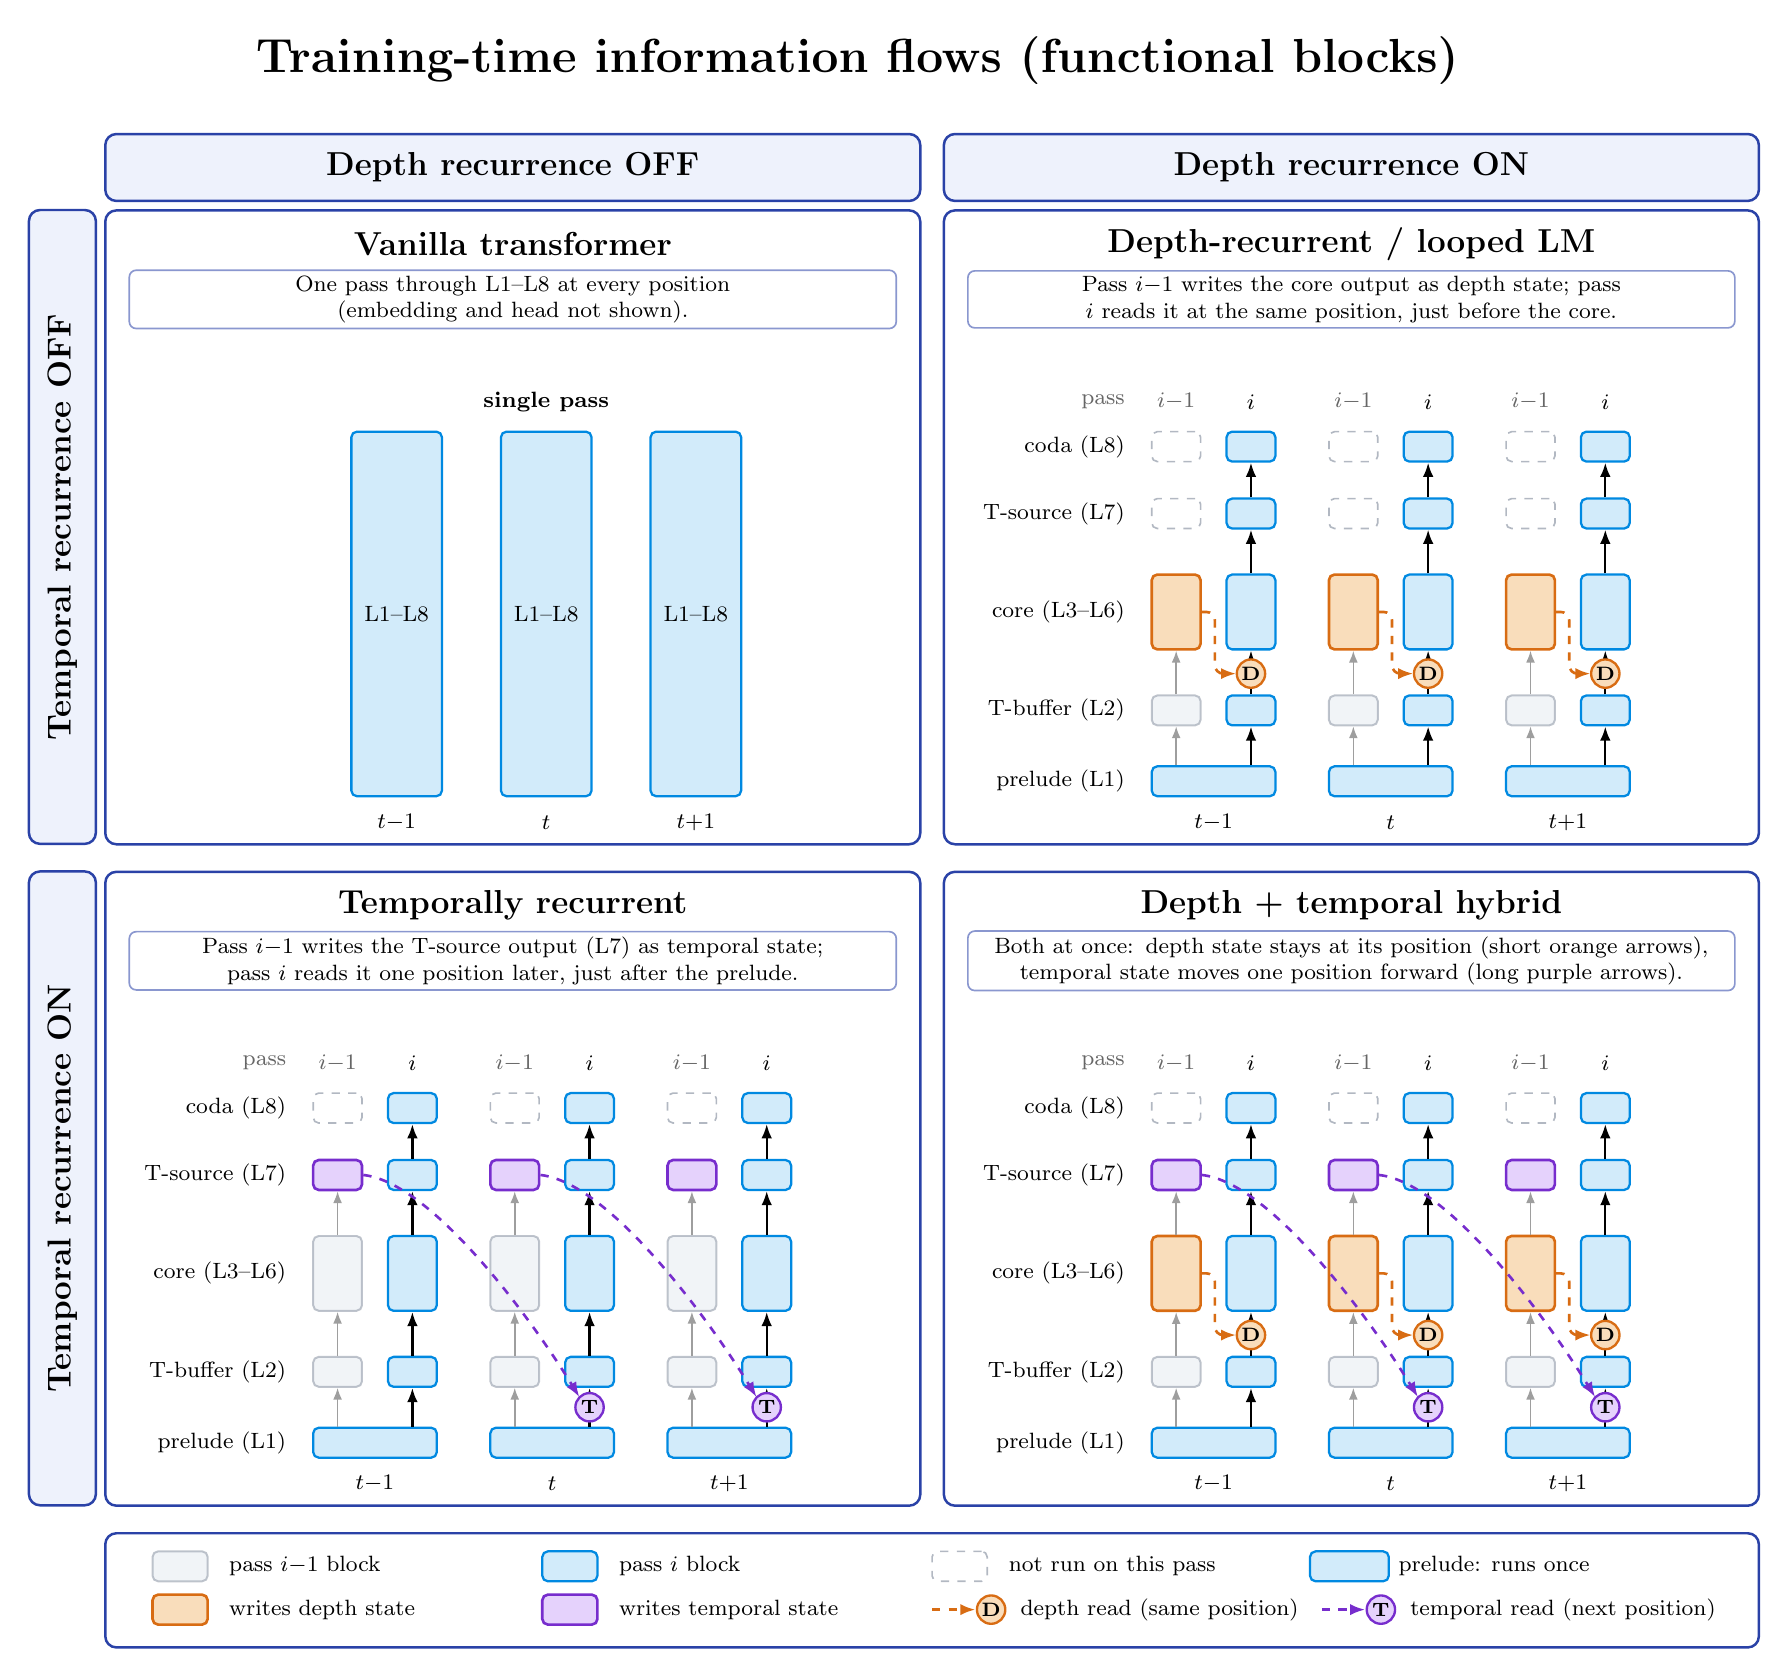
\begin{tikzpicture}[x=1cm,y=1cm]

\node[font=\bfseries\LARGE] at (11.9,17.30) {Training-time information flows (functional blocks)};
\node[header, minimum width=10.35cm, minimum height=0.85cm, font=\bfseries\large] at (7.525,15.945) {Depth recurrence OFF};
\node[header, minimum width=10.35cm, minimum height=0.85cm, font=\bfseries\large] at (18.175,15.945) {Depth recurrence ON};
\node[sideheader, minimum width=8.05cm, minimum height=0.85cm, rotate=90, font=\bfseries\large] at (1.805,11.38) {Temporal recurrence OFF};
\node[sideheader, minimum width=8.05cm, minimum height=0.85cm, rotate=90, font=\bfseries\large] at (1.805,2.98) {Temporal recurrence ON};

% ---------------- Vanilla transformer
\begin{scope}[shift={(2.35,7.35)}]
  \draw[panel] (0,0) rectangle (10.35,8.05);
  \node[font=\bfseries\large] at (5.175,7.62) {Vanilla transformer};
  \node[descbox, text width=9.6cm] at (5.175,6.92) {One pass through L1--L8 at every position (embedding and head not shown).};
  \node[font=\bfseries\footnotesize] at (5.60,5.62) {single pass};
  \node[active, minimum height=4.63cm, minimum width=1.15cm, font=\footnotesize] (tlc0) at (3.700,2.925) {L1--L8};
  \node[font=\footnotesize] at (3.7,0.28) {$t{-}1$};
  \node[active, minimum height=4.63cm, minimum width=1.15cm, font=\footnotesize] (tlc1) at (5.600,2.925) {L1--L8};
  \node[font=\footnotesize] at (5.6,0.28) {$t$};
  \node[active, minimum height=4.63cm, minimum width=1.15cm, font=\footnotesize] (tlc2) at (7.500,2.925) {L1--L8};
  \node[font=\footnotesize] at (7.5,0.28) {$t{+}1$};
\end{scope}

% ---------------- Depth-recurrent / looped LM
\begin{scope}[shift={(13.0,7.35)}]
  \draw[panel] (0,0) rectangle (10.35,8.05);
  \node[font=\bfseries\large] at (5.175,7.62) {Depth-recurrent / looped LM};
  \node[descbox, text width=9.6cm] at (5.175,6.92) {Pass $i{-}1$ writes the core output as depth state; pass $i$ reads it at the same position, just before the core.};
  \node[anchor=east, font=\footnotesize] at (2.42,0.8) {prelude (L1)};
  \node[anchor=east, font=\footnotesize] at (2.42,1.7) {T-buffer (L2)};
  \node[anchor=east, font=\footnotesize] at (2.42,2.95) {core (L3--L6)};
  \node[anchor=east, font=\footnotesize] at (2.42,4.2) {T-source (L7)};
  \node[anchor=east, font=\footnotesize] at (2.42,5.05) {coda (L8)};
  \node[anchor=east, font=\footnotesize, text=black!60] at (2.42,5.62) {pass};
  \node[font=\footnotesize, text=black!60] at (2.95,5.62) {$i{-}1$};
  \node[font=\bfseries\footnotesize] at (3.9000000000000004,5.62) {$i$};
  \node[active, minimum width=1.5699999999999998cm] (trpre0) at (3.425,0.800) {};
  \node[ghost] (trp0b2) at (2.950,1.700) {};
  \draw[ghostflow] (trpre0.north -| trp0b2) -- (trp0b2.south);
  \node[depthmark, minimum height=0.95cm] (trp0b3) at (2.950,2.950) {};
  \draw[ghostflow] (trp0b2.north) -- (trp0b3.south);
  \node[notrun] (trp0b4) at (2.950,4.200) {};
  \node[notrun] (trp0b5) at (2.950,5.050) {};
  \node[active] (trq0b2) at (3.900,1.700) {};
  \node[active, minimum height=0.95cm] (trq0b3) at (3.900,2.950) {};
  \node[active] (trq0b4) at (3.900,4.200) {};
  \node[active] (trq0b5) at (3.900,5.050) {};
  \draw[flow] (trpre0.north -| trq0b2) -- (trq0b2.south);
  \draw[flow] (trq0b2.north) -- (trq0b3.south);
  \draw[flow] (trq0b3.north) -- (trq0b4.south);
  \draw[flow] (trq0b4.north) -- (trq0b5.south);
  \node[font=\footnotesize] at (3.4250000000000003,0.28) {$t{-}1$};
  \node[font=\footnotesize, text=black!60] at (5.2,5.62) {$i{-}1$};
  \node[font=\bfseries\footnotesize] at (6.15,5.62) {$i$};
  \node[active, minimum width=1.5699999999999998cm] (trpre1) at (5.675,0.800) {};
  \node[ghost] (trp1b2) at (5.200,1.700) {};
  \draw[ghostflow] (trpre1.north -| trp1b2) -- (trp1b2.south);
  \node[depthmark, minimum height=0.95cm] (trp1b3) at (5.200,2.950) {};
  \draw[ghostflow] (trp1b2.north) -- (trp1b3.south);
  \node[notrun] (trp1b4) at (5.200,4.200) {};
  \node[notrun] (trp1b5) at (5.200,5.050) {};
  \node[active] (trq1b2) at (6.150,1.700) {};
  \node[active, minimum height=0.95cm] (trq1b3) at (6.150,2.950) {};
  \node[active] (trq1b4) at (6.150,4.200) {};
  \node[active] (trq1b5) at (6.150,5.050) {};
  \draw[flow] (trpre1.north -| trq1b2) -- (trq1b2.south);
  \draw[flow] (trq1b2.north) -- (trq1b3.south);
  \draw[flow] (trq1b3.north) -- (trq1b4.south);
  \draw[flow] (trq1b4.north) -- (trq1b5.south);
  \node[font=\footnotesize] at (5.675000000000001,0.28) {$t$};
  \node[font=\footnotesize, text=black!60] at (7.45,5.62) {$i{-}1$};
  \node[font=\bfseries\footnotesize] at (8.4,5.62) {$i$};
  \node[active, minimum width=1.5699999999999998cm] (trpre2) at (7.925,0.800) {};
  \node[ghost] (trp2b2) at (7.450,1.700) {};
  \draw[ghostflow] (trpre2.north -| trp2b2) -- (trp2b2.south);
  \node[depthmark, minimum height=0.95cm] (trp2b3) at (7.450,2.950) {};
  \draw[ghostflow] (trp2b2.north) -- (trp2b3.south);
  \node[notrun] (trp2b4) at (7.450,4.200) {};
  \node[notrun] (trp2b5) at (7.450,5.050) {};
  \node[active] (trq2b2) at (8.400,1.700) {};
  \node[active, minimum height=0.95cm] (trq2b3) at (8.400,2.950) {};
  \node[active] (trq2b4) at (8.400,4.200) {};
  \node[active] (trq2b5) at (8.400,5.050) {};
  \draw[flow] (trpre2.north -| trq2b2) -- (trq2b2.south);
  \draw[flow] (trq2b2.north) -- (trq2b3.south);
  \draw[flow] (trq2b3.north) -- (trq2b4.south);
  \draw[flow] (trq2b4.north) -- (trq2b5.south);
  \node[font=\footnotesize] at (7.925000000000001,0.28) {$t{+}1$};
  \draw[dread, rounded corners=3pt] (trp0b3.east) -- ++(0.165,0) |- (3.710,2.167);
  \node[injectD] at (3.900,2.167) {D};
  \draw[dread, rounded corners=3pt] (trp1b3.east) -- ++(0.165,0) |- (5.960,2.167);
  \node[injectD] at (6.150,2.167) {D};
  \draw[dread, rounded corners=3pt] (trp2b3.east) -- ++(0.165,0) |- (8.210,2.167);
  \node[injectD] at (8.400,2.167) {D};
\end{scope}

% ---------------- Temporally recurrent
\begin{scope}[shift={(2.35,-1.05)}]
  \draw[panel] (0,0) rectangle (10.35,8.05);
  \node[font=\bfseries\large] at (5.175,7.62) {Temporally recurrent};
  \node[descbox, text width=9.6cm] at (5.175,6.92) {Pass $i{-}1$ writes the T-source output (L7) as temporal state; pass $i$ reads it one position later, just after the prelude.};
  \node[anchor=east, font=\footnotesize] at (2.42,0.8) {prelude (L1)};
  \node[anchor=east, font=\footnotesize] at (2.42,1.7) {T-buffer (L2)};
  \node[anchor=east, font=\footnotesize] at (2.42,2.95) {core (L3--L6)};
  \node[anchor=east, font=\footnotesize] at (2.42,4.2) {T-source (L7)};
  \node[anchor=east, font=\footnotesize] at (2.42,5.05) {coda (L8)};
  \node[anchor=east, font=\footnotesize, text=black!60] at (2.42,5.62) {pass};
  \node[font=\footnotesize, text=black!60] at (2.95,5.62) {$i{-}1$};
  \node[font=\bfseries\footnotesize] at (3.9000000000000004,5.62) {$i$};
  \node[active, minimum width=1.5699999999999998cm] (blpre0) at (3.425,0.800) {};
  \node[ghost] (blp0b2) at (2.950,1.700) {};
  \draw[ghostflow] (blpre0.north -| blp0b2) -- (blp0b2.south);
  \node[ghost, minimum height=0.95cm] (blp0b3) at (2.950,2.950) {};
  \draw[ghostflow] (blp0b2.north) -- (blp0b3.south);
  \node[tempmark] (blp0b4) at (2.950,4.200) {};
  \draw[ghostflow] (blp0b3.north) -- (blp0b4.south);
  \node[notrun] (blp0b5) at (2.950,5.050) {};
  \node[active] (blq0b2) at (3.900,1.700) {};
  \node[active, minimum height=0.95cm] (blq0b3) at (3.900,2.950) {};
  \node[active] (blq0b4) at (3.900,4.200) {};
  \node[active] (blq0b5) at (3.900,5.050) {};
  \draw[flow] (blpre0.north -| blq0b2) -- (blq0b2.south);
  \draw[flow] (blq0b2.north) -- (blq0b3.south);
  \draw[flow] (blq0b3.north) -- (blq0b4.south);
  \draw[flow] (blq0b4.north) -- (blq0b5.south);
  \node[font=\footnotesize] at (3.4250000000000003,0.28) {$t{-}1$};
  \node[font=\footnotesize, text=black!60] at (5.2,5.62) {$i{-}1$};
  \node[font=\bfseries\footnotesize] at (6.15,5.62) {$i$};
  \node[active, minimum width=1.5699999999999998cm] (blpre1) at (5.675,0.800) {};
  \node[ghost] (blp1b2) at (5.200,1.700) {};
  \draw[ghostflow] (blpre1.north -| blp1b2) -- (blp1b2.south);
  \node[ghost, minimum height=0.95cm] (blp1b3) at (5.200,2.950) {};
  \draw[ghostflow] (blp1b2.north) -- (blp1b3.south);
  \node[tempmark] (blp1b4) at (5.200,4.200) {};
  \draw[ghostflow] (blp1b3.north) -- (blp1b4.south);
  \node[notrun] (blp1b5) at (5.200,5.050) {};
  \node[active] (blq1b2) at (6.150,1.700) {};
  \node[active, minimum height=0.95cm] (blq1b3) at (6.150,2.950) {};
  \node[active] (blq1b4) at (6.150,4.200) {};
  \node[active] (blq1b5) at (6.150,5.050) {};
  \draw[flow] (blpre1.north -| blq1b2) -- (blq1b2.south);
  \draw[flow] (blq1b2.north) -- (blq1b3.south);
  \draw[flow] (blq1b3.north) -- (blq1b4.south);
  \draw[flow] (blq1b4.north) -- (blq1b5.south);
  \node[font=\footnotesize] at (5.675000000000001,0.28) {$t$};
  \node[font=\footnotesize, text=black!60] at (7.45,5.62) {$i{-}1$};
  \node[font=\bfseries\footnotesize] at (8.4,5.62) {$i$};
  \node[active, minimum width=1.5699999999999998cm] (blpre2) at (7.925,0.800) {};
  \node[ghost] (blp2b2) at (7.450,1.700) {};
  \draw[ghostflow] (blpre2.north -| blp2b2) -- (blp2b2.south);
  \node[ghost, minimum height=0.95cm] (blp2b3) at (7.450,2.950) {};
  \draw[ghostflow] (blp2b2.north) -- (blp2b3.south);
  \node[tempmark] (blp2b4) at (7.450,4.200) {};
  \draw[ghostflow] (blp2b3.north) -- (blp2b4.south);
  \node[notrun] (blp2b5) at (7.450,5.050) {};
  \node[active] (blq2b2) at (8.400,1.700) {};
  \node[active, minimum height=0.95cm] (blq2b3) at (8.400,2.950) {};
  \node[active] (blq2b4) at (8.400,4.200) {};
  \node[active] (blq2b5) at (8.400,5.050) {};
  \draw[flow] (blpre2.north -| blq2b2) -- (blq2b2.south);
  \draw[flow] (blq2b2.north) -- (blq2b3.south);
  \draw[flow] (blq2b3.north) -- (blq2b4.south);
  \draw[flow] (blq2b4.north) -- (blq2b5.south);
  \node[font=\footnotesize] at (7.925000000000001,0.28) {$t{+}1$};
  \draw[tread] (blp0b4.east) .. controls +(0.9,-0.1) and +(-0.55,0.9) .. (6.020,1.380);
  \node[injectT] at (6.150,1.250) {T};
  \draw[tread] (blp1b4.east) .. controls +(0.9,-0.1) and +(-0.55,0.9) .. (8.270,1.380);
  \node[injectT] at (8.400,1.250) {T};
\end{scope}

% ---------------- Depth + temporal hybrid
\begin{scope}[shift={(13.0,-1.05)}]
  \draw[panel] (0,0) rectangle (10.35,8.05);
  \node[font=\bfseries\large] at (5.175,7.62) {Depth + temporal hybrid};
  \node[descbox, text width=9.6cm] at (5.175,6.92) {Both at once: depth state stays at its position (short orange arrows), temporal state moves one position forward (long purple arrows).};
  \node[anchor=east, font=\footnotesize] at (2.42,0.8) {prelude (L1)};
  \node[anchor=east, font=\footnotesize] at (2.42,1.7) {T-buffer (L2)};
  \node[anchor=east, font=\footnotesize] at (2.42,2.95) {core (L3--L6)};
  \node[anchor=east, font=\footnotesize] at (2.42,4.2) {T-source (L7)};
  \node[anchor=east, font=\footnotesize] at (2.42,5.05) {coda (L8)};
  \node[anchor=east, font=\footnotesize, text=black!60] at (2.42,5.62) {pass};
  \node[font=\footnotesize, text=black!60] at (2.95,5.62) {$i{-}1$};
  \node[font=\bfseries\footnotesize] at (3.9000000000000004,5.62) {$i$};
  \node[active, minimum width=1.5699999999999998cm] (brpre0) at (3.425,0.800) {};
  \node[ghost] (brp0b2) at (2.950,1.700) {};
  \draw[ghostflow] (brpre0.north -| brp0b2) -- (brp0b2.south);
  \node[depthmark, minimum height=0.95cm] (brp0b3) at (2.950,2.950) {};
  \draw[ghostflow] (brp0b2.north) -- (brp0b3.south);
  \node[tempmark] (brp0b4) at (2.950,4.200) {};
  \draw[ghostflow] (brp0b3.north) -- (brp0b4.south);
  \node[notrun] (brp0b5) at (2.950,5.050) {};
  \node[active] (brq0b2) at (3.900,1.700) {};
  \node[active, minimum height=0.95cm] (brq0b3) at (3.900,2.950) {};
  \node[active] (brq0b4) at (3.900,4.200) {};
  \node[active] (brq0b5) at (3.900,5.050) {};
  \draw[flow] (brpre0.north -| brq0b2) -- (brq0b2.south);
  \draw[flow] (brq0b2.north) -- (brq0b3.south);
  \draw[flow] (brq0b3.north) -- (brq0b4.south);
  \draw[flow] (brq0b4.north) -- (brq0b5.south);
  \node[font=\footnotesize] at (3.4250000000000003,0.28) {$t{-}1$};
  \node[font=\footnotesize, text=black!60] at (5.2,5.62) {$i{-}1$};
  \node[font=\bfseries\footnotesize] at (6.15,5.62) {$i$};
  \node[active, minimum width=1.5699999999999998cm] (brpre1) at (5.675,0.800) {};
  \node[ghost] (brp1b2) at (5.200,1.700) {};
  \draw[ghostflow] (brpre1.north -| brp1b2) -- (brp1b2.south);
  \node[depthmark, minimum height=0.95cm] (brp1b3) at (5.200,2.950) {};
  \draw[ghostflow] (brp1b2.north) -- (brp1b3.south);
  \node[tempmark] (brp1b4) at (5.200,4.200) {};
  \draw[ghostflow] (brp1b3.north) -- (brp1b4.south);
  \node[notrun] (brp1b5) at (5.200,5.050) {};
  \node[active] (brq1b2) at (6.150,1.700) {};
  \node[active, minimum height=0.95cm] (brq1b3) at (6.150,2.950) {};
  \node[active] (brq1b4) at (6.150,4.200) {};
  \node[active] (brq1b5) at (6.150,5.050) {};
  \draw[flow] (brpre1.north -| brq1b2) -- (brq1b2.south);
  \draw[flow] (brq1b2.north) -- (brq1b3.south);
  \draw[flow] (brq1b3.north) -- (brq1b4.south);
  \draw[flow] (brq1b4.north) -- (brq1b5.south);
  \node[font=\footnotesize] at (5.675000000000001,0.28) {$t$};
  \node[font=\footnotesize, text=black!60] at (7.45,5.62) {$i{-}1$};
  \node[font=\bfseries\footnotesize] at (8.4,5.62) {$i$};
  \node[active, minimum width=1.5699999999999998cm] (brpre2) at (7.925,0.800) {};
  \node[ghost] (brp2b2) at (7.450,1.700) {};
  \draw[ghostflow] (brpre2.north -| brp2b2) -- (brp2b2.south);
  \node[depthmark, minimum height=0.95cm] (brp2b3) at (7.450,2.950) {};
  \draw[ghostflow] (brp2b2.north) -- (brp2b3.south);
  \node[tempmark] (brp2b4) at (7.450,4.200) {};
  \draw[ghostflow] (brp2b3.north) -- (brp2b4.south);
  \node[notrun] (brp2b5) at (7.450,5.050) {};
  \node[active] (brq2b2) at (8.400,1.700) {};
  \node[active, minimum height=0.95cm] (brq2b3) at (8.400,2.950) {};
  \node[active] (brq2b4) at (8.400,4.200) {};
  \node[active] (brq2b5) at (8.400,5.050) {};
  \draw[flow] (brpre2.north -| brq2b2) -- (brq2b2.south);
  \draw[flow] (brq2b2.north) -- (brq2b3.south);
  \draw[flow] (brq2b3.north) -- (brq2b4.south);
  \draw[flow] (brq2b4.north) -- (brq2b5.south);
  \node[font=\footnotesize] at (7.925000000000001,0.28) {$t{+}1$};
  \draw[dread, rounded corners=3pt] (brp0b3.east) -- ++(0.165,0) |- (3.710,2.167);
  \node[injectD] at (3.900,2.167) {D};
  \draw[dread, rounded corners=3pt] (brp1b3.east) -- ++(0.165,0) |- (5.960,2.167);
  \node[injectD] at (6.150,2.167) {D};
  \draw[tread] (brp0b4.east) .. controls +(0.9,-0.1) and +(-0.55,0.9) .. (6.020,1.380);
  \node[injectT] at (6.150,1.250) {T};
  \draw[dread, rounded corners=3pt] (brp2b3.east) -- ++(0.165,0) |- (8.210,2.167);
  \node[injectD] at (8.400,2.167) {D};
  \draw[tread] (brp1b4.east) .. controls +(0.9,-0.1) and +(-0.55,0.9) .. (8.270,1.380);
  \node[injectT] at (8.400,1.250) {T};
\end{scope}

% ---------------- Legend
\begin{scope}[shift={(2.35,-2.85)}]
  \draw[panel] (0,0) rectangle (21.00,1.45);
  \node[ghost, minimum width=0.70cm] at (0.95,1.03) {};
  \node[legendtext] at (1.45,1.03) {pass $i{-}1$ block};
  \node[active, minimum width=0.70cm] at (5.90,1.03) {};
  \node[legendtext] at (6.40,1.03) {pass $i$ block};
  \node[notrun, minimum width=0.70cm] at (10.85,1.03) {};
  \node[legendtext] at (11.35,1.03) {not run on this pass};
  \node[active, minimum width=1.0cm] at (15.80,1.03) {};
  \node[legendtext] at (16.30,1.03) {prelude: runs once};
  \node[depthmark, minimum width=0.70cm] at (0.95,0.48) {};
  \node[legendtext] at (1.45,0.48) {writes depth state};
  \node[tempmark, minimum width=0.70cm] at (5.90,0.48) {};
  \node[legendtext] at (6.40,0.48) {writes temporal state};
  \draw[dread] (10.50,0.48) -- (11.05,0.48);
  \node[injectD] at (11.25,0.48) {D};
  \node[legendtext] at (11.50,0.48) {depth read (same position)};
  \draw[tread] (15.45,0.48) -- (16.00,0.48);
  \node[injectT] at (16.20,0.48) {T};
  \node[legendtext] at (16.45,0.48) {temporal read (next position)};
\end{scope}
\end{tikzpicture}
\end{document}
